\section{The Scientific Procedure} \index{Scientific Procedure}

%\begin{multicols}{2}


\subsection{Acids and Bases} \index{Acids and bases}

\begin{center}
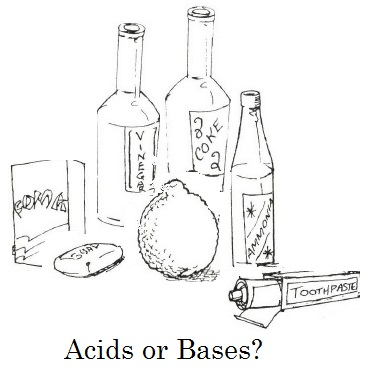
\includegraphics[width=0.4\textwidth]{./img/source/acids-bases-sci-meth.jpg}
\end{center}

\begin{description*}
\item[Materials:]{Bottles, bottle caps, water, vinegar, lemons, baking soda, soda, soap, antacid tablets, rosella leaves, straws/syringes}
\item[Setup:]{Prepare solutions for each of the items above in separate bottles. Prepare indicator by placing rosella leaves in hot water.}\\
\item[Problem:]{What differences can we observe among acids and bases?\\

\begin{tabular}{|l|c|c|} \hline
\multirow{2}{*}{\textbf{Solutions}} & \textbf{Hypothesis} & \multirow{2}{*}{\textbf{Experimental Result}} \\
& \textbf{(Which is different?)} & \\ \hline
Vinegar, lemon, baking soda & & \\ \hline
Vinegar, baking soda, soap & & \\ \hline
Baking soda, antacid, soda & & \\ \hline
Soda, soap, vinegar & & \\ \hline
\end{tabular} \\[10pt]
}
\item[Hypothesis:]{For each set of solutions, which one will reveal a colour different from the others? Record your predictions in the table.}
\item[Procedure:]{Place small amounts of 3 different solutions in separate bottle caps according to the table. Add a few drops of rosella indicator to each.}
\item[Observations:]{Record observations of colour change under \emph{Experimental Result} in the table.}
\item[Questions:]{\hfill
\begin{enumerate}
\item Which solutions have similar properties?
\item Which solutions are acids? What colour do they show?
\item Which solutions are bases? What colour do they show?
\end{enumerate}
}
\item[Theory:]{Coloured leaves such as rosella act as indicators for identifying acids and bases. Adding rosella indicator reveals a red colour for acids and a blue colour for bases. Students do not need to understand the differences between acids and bases in order to observe their different behaviours. Locally available examples of acids include sour milk, citrus fruits and soda. Local bases include ammonia, toothpaste and detergent.}
\end{description*}


\subsection{Mixing Acids and Bases}

\begin{center}
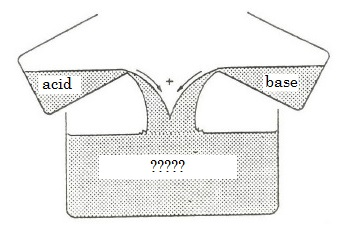
\includegraphics[width=0.6\textwidth]{./img/source/mixing-acid-base.jpg}
\end{center}

\begin{description*}
\item[Problem:]{What happens when acids and bases are mixed together?\\

\begin{tabular}{|l|c|c|} \hline
\multirow{2}{*}{\textbf{Solutions to Mix}} & \textbf{Hypothesis} & \multirow{2}{*}{\textbf{Experimental Result}} \\
& \textbf{(What colour?)} & \\ \hline
Mix vinegar and lemon & & \\ \hline
Mix baking soda and soap & & \\ \hline
Mix vinegar and baking soda & & \\ \hline
\end{tabular}\\[10pt]
}
\item[Hypothesis:]{Predict any colour changes or observations when pairs of solutions are mixed together. Record in the table.}
\item[Procedure:]{Mix small amounts of solutions together according to the table.}
\item[Observations:]{Record observations (colour changes, etc.) in the table.}
\item[Questions:]{\hfill
\begin{enumerate}
\item What happens when an acid is mixed with an acid?
\item What happens when a base is mixed with a base?
\item What happens when an acid is mixed with a base?
\end{enumerate}
}
\item[Theory:]{Mixing acids with acids and bases with bases may cause the colour of the solution to turn darker or lighter depending on the solutions used. Mixing an acid with a base should reveal a colourless solution and produce carbon dioxide gas. You may need to vary the amounts of acid and base to get a colourless solution depending on their concentrations.}
\end{description*}

%==================================================================================================%


%\end{multicols}

\pagebreak